\subsection{Unlocking Antenna Power: Comparing Gain to a Half-Wavelength Dipole!}

\begin{tcolorbox}[colback=gray!10, colframe=black, title=E9A12] How much gain does an antenna have compared to a half-wavelength dipole if it has 6 dB gain over an isotropic radiator? 

\begin{enumerate}[label=\Alph*.]
    \item 3.85 dB
    \item \textbf{6.0 dB}
    \item 8.15 dB
    \item 2.79 dB
\end{enumerate} \end{tcolorbox}

\subsubsection{Concepts Involved}

To solve this question, we need to understand the concept of antenna gain and the reference points used for comparison. 

1. \textbf{Antenna Gain:}: Gain is a measure of how well an antenna converts input power into radio waves in a specified direction. It is often expressed in decibels (dB).

2. \textbf{Isotropic Radiator:}: This is a hypothetical antenna that radiates power equally in all directions. It is often used as a baseline reference point for measuring gain.

3. \textbf{Half-Wavelength Dipole:}: This is a practical antenna which has a gain of approximately 2.15 dB over an isotropic radiator.

Now, if the antenna has a gain of 6 dB over an isotropic radiator, we can determine its gain relative to the half-wavelength dipole.

\subsubsection{Calculation Steps}

1. We find the actual gain of the antenna relative to the isotropic radiator, which is given as 6 dB.
   
2. We factor in the gain of the half-wavelength dipole:
   \[
   \text{Gain of Dipole} = 2.15 \, \text{dB}
   \]

3. The gain of the antenna compared to the dipole is then calculated by subtracting the gain of the half-wavelength dipole from the gain of the antenna compared to the isotropic radiator:
   \[
   \text{Gain compared to Dipole} = \text{Gain (Antenna)} - \text{Gain (Dipole)} 
   \]
   \[
   = 6 \, \text{dB} - 2.15 \, \text{dB} = 3.85 \, \text{dB}
   \]

Thus, the gain of this antenna compared to a half-wavelength dipole is 3.85 dB.

\subsubsection{Conclusion}

The answer to the question is therefore option A: 3.85 dB. 

This illustrates an important concept in antenna design and radio communication: assessing performance relative to standard antennas, like the half-wavelength dipole, helps engineers predict how a new antenna will perform in real-world applications. 

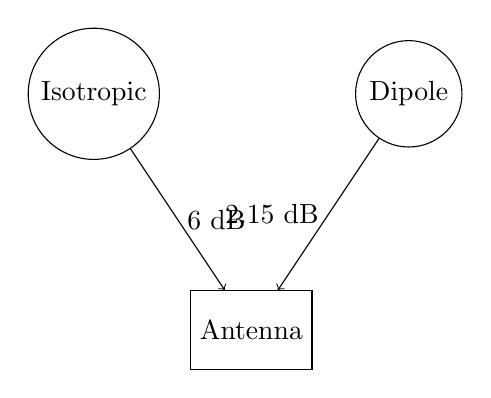
\begin{tikzpicture}
    \node at (0,0) [draw, circle, minimum size=1cm] (iso) {Isotropic};
    \node at (4,0) [draw, circle, minimum size=1cm] (dipole) {Dipole};
    \node at (2,-3) [draw, rectangle, minimum width=1cm, minimum height=1cm] (antenna) {Antenna};
    \draw[->] (iso) -- (antenna) node[midway, right] {6 dB};
    \draw[->] (dipole) -- (antenna) node[midway, left] {2.15 dB};
\end{tikzpicture}